\documentclass[
paper=A4,
pagesize,
abstract,
11pt,
titlepage,
BCOR=12mm,
twoside,
footinclude=false,
headinclude=false
]{scrreprt}

% Personal data and user ad-hoc commands
\newcommand*{\mydegree}{M.Sc.}
\newcommand*{\myname}{Bastian Leykauf}
\newcommand*{\mylocation}{Berlin}
\newcommand*{\mytime}{\today}

% Font and language setup
\usepackage{fontspec}

% math and scientific packages
\usepackage{mathtools}
\usepackage[
    math-style=ISO,
    bold-style=ISO,
    partial=upright,
    nabla=upright
]{unicode-math}

%fonts and languages

\setmainfont{LibertinusSerif}[
    UprightFont    = *-Regular,
    BoldFont       = *-Bold,
    ItalicFont     = *-Italic,
    BoldItalicFont = *-BoldItalic,
    Ligatures      = TeX,
    Extension      = .otf,
    Path           = fonts/
]

\setsansfont{LibertinusSans}[
     UprightFont    = *-Regular,
     BoldFont       = *-Bold,
     ItalicFont     = *-Italic,
     Ligatures      = TeX,
     Extension      = .otf,
     Path           = fonts/
]

\setmathfont{LibertinusMath-Regular}[
    Extension       = .otf,
    Path            = fonts/
]

%\setmonofont{LibertinusMono-Regular}[
\setmonofont{Inconsolata-Regular}[ % Inconsolata looks better than the Libertinus Mono font
    Extension      = .otf,
    Path           = fonts/
]

\usepackage{microtype}                       	% slightly tweak font spacing for aesthetics
\usepackage{polyglossia}
\setdefaultlanguage{english}
\setotherlanguage{german}

% references
\usepackage[hidelinks]{hyperref}
\usepackage{cleveref}

\usepackage{csquotes}        % quotes

\usepackage[acronym, nomain, nonumberlist, nogroupskip, automake]{glossaries} %for glossary
\usepackage{glossary-mcols}
\newacronym{aom}{AOM}{acousto-optic modulator}
\newacronym{bkg}{BKG}{Bundesamt für Kartographie und Geodäsie, engl. \emph{Federal Agency for Cartography and Geodesy}}
\newacronym{cad}{CAD}{computer-aided design}
\newacronym{ccd}{CCD}{charge-coupled device}
\newacronym{cmos}{CMOS}{Complementary metal-oxide-semiconductor}
\newacronym{codata}{CODATA}{Committee on Data of the International Council for Science}
\newacronym{dds}{DDS}{direct digital synthesizer}
\newacronym{dfb}{DFB}{distributed feedback}
\newacronym{dro}{DRO}{dielectric resonator oscillator}
\newacronym{ecdl}{ECDL}{external cavity diode laser}
\newacronym{fem}{FEM}{finite element method}
\newacronym{fwhm}{FWHM}{full width half maximum}
\newacronym{gps}{GPS}{Global Positioning System}
\newacronym{mot}{MOT}{magneto-optical trap}
\newacronym{mts}{MTS}{modulation transfer spectroscopy}
\newacronym{pbs}{PBS}{polarizing beamsplitter}
\newacronym{pfd}{PFD}{phase-frequency detector}
\newacronym{pid}{PID}{proportional–integral–derivative}
\newacronym{pll}{PLL}{phase-locked loop}
\newacronym{pmt}{PMT}{photo-multiplier tube}
\newacronym{psd}{PSD}{power spectral density}
\newacronym{rms}{RMS}{root mean square}
\newacronym{si}{SI}{Système international}
\newacronym{ta}{TA}{tapered amplifier}
\newacronym{uhv}{UHV}{ultra-high vacuum}
\makeglossaries

% bibliography
\usepackage[style=phys,
				biblabel=brackets,
				doi=true,
				url=true,
				giveninits=true,
				hyperref,
				eprint=true,
				backend=biber]{biblatex}
\addbibresource{bibliography.bib}

% Tables, (sub)figures, and captions, URLs
\usepackage{tabularx}
\usepackage{booktabs}                                         % Horizontal rules in tables
\usepackage[normal]{threeparttable}         		       	% notes in tables
    \usepackage{etoolbox}                                       % fixes bug with threeparttable and situnitx
      \robustify\tnote                                          %
\usepackage{longtable}
\usepackage{caption}
\addtokomafont{caption}{\small}
\setcapindent{1em}
\usepackage{url}                    % typesetting URLs
\usepackage{graphicx}
\graphicspath{ {graphics/}}

% units
\usepackage[locale=US,mode=math]{siunitx}
    \sisetup{separate-uncertainty = true,        % use \pm for seperating value and uncertainty
    			 math-micro=\text{µ}, text-micro=µ}  % micro doesn't work with XeTeX otherwise

\usepackage{braket}                           % Dirac bras, kets and brakets
\usepackage{bropd}                            % automatic bracket matching and differential operators
\usepackage[version=3]{mhchem}                % chemical molecular formulae and chemical equations   

% Layout stuff
\usepackage[draft]{todonotes}
\usepackage{epigraph}

%\widowpenalty10000
%\clubpenalty100000
% Custom commands

% mathematics
\renewcommand*{\vec}{\mathbfit}
\newcommand*{\tensor}{\mathbfsf}
\newcommand*{\mtrx}[1]{\mathbf{#1}}                            % matrices are upright boldface
\newcommand*{\e}{\mathrm{e}}                                   % Euler's number
\renewcommand*{\i}{\mathrm{i}}                                 % imaginary unit
\renewcommand*{\pi}{\uppi}                                     % pi is a constant
\DeclareMathOperator{\const}{const.}                           % constant

%\newcommand*\mean[1]{\bar{#1}}                                 % mean value
\DeclareMathOperator{\diag}{diag}                              % diagonal elements
%\newcommand*{\transpose}{\intercal}                            % matrix transpose
\DeclareMathOperator{\sgn}{sgn}                                % sign operator
\DeclareMathOperator{\Tr}{Tr}

% physics
\newcommand*{\Del}[1]{\mathop{}\!\increment #1\mathop{}\!}     % fix spacing for delta, denoting differences (delta x = x_2 - x_1)
\newcommand*{\kb}{k_\text{b}}                                  % Boltzmann constant
\newcommand*{\op}{\hat}                                        % quantum mechanical operators
\newcommand*{\snr}{\mathit{SNR}}

% declare new units
\DeclareSIUnit\Gal{Gal}
\DeclareSIUnit{\E}{E}
\DeclareSIUnit{\sqrthz}{\hertz\tothe{1/2}}

\newcommand{\code}{\texttt}

\makeglossary

\begin{document}
\pagenumbering{roman}
\pagestyle{plain}
\titlehead{
   \centering
      {\Large\myuniversity\\
       \textit{\myfaculty}}
}
       
\title{\mytitle}
\subtitle{\mysubtitle}
\date{\mytime}
\author{\myname, \mydegree}
\publishers{
   \begin{flushleft}
      Gutachter:\\
         \myprof\\
         \myotherprof  
   \end{flushleft}
}

\maketitle


\begin{german}
   \begin{abstract}
      Das ist die Zusammenfassung.
   \end{abstract}
\end{german}


\begin{abstract}
   This is the abstract.
\end{abstract}



\KOMAoption{listof}{leveldown}

\tableofcontents
\listoffigures
\listoftables
\cleardoublepage



\cleardoublepage
\printglossary
\label{app:acronyms} 

\pagestyle{headings}
\pagenumbering{arabic}
\chapter{Introduction}\label{ch:introduction}
This thesis presents some interesting physics, complete with numbers
\begin{equation}
	g = \SI{100+-1}{kg}\text{,}
\end{equation}
chemical formulae like \ce{^{87}Rb} and some other nonsense:
\begin{equation}
	\Delta x = x_1 - x_2
\end{equation}
\begin{equation}
	\vec{x}
\end{equation}

Note that the imaginary number and Euler's number and $\pi$ are not set in italics since they are mathematical constants:
\begin{equation}
	\e^{\i\pi} - 1 = 0\text{.}
\end{equation}

Some more advanced stuff:
\begin{subequations}\label{eq:schroedinger}
	\begin{gather}
		\i \hbar \pd{}{t}\Phi = \op{H}\Phi\\
		E\Phi(\vec{r}) = \br{\frac{-\hbar^2}{2m} \nabla^2 + V(\vec{r}) } \Phi(\vec{r})
	\end{gather}
\end{subequations}

\section{Text width}
For drawing figures, it can be useful to know the textwidth and height. In this document, the text is \the\textwidth {} wide and \the\textheight {} high.

\begin{figure}[tb]
	\centering
	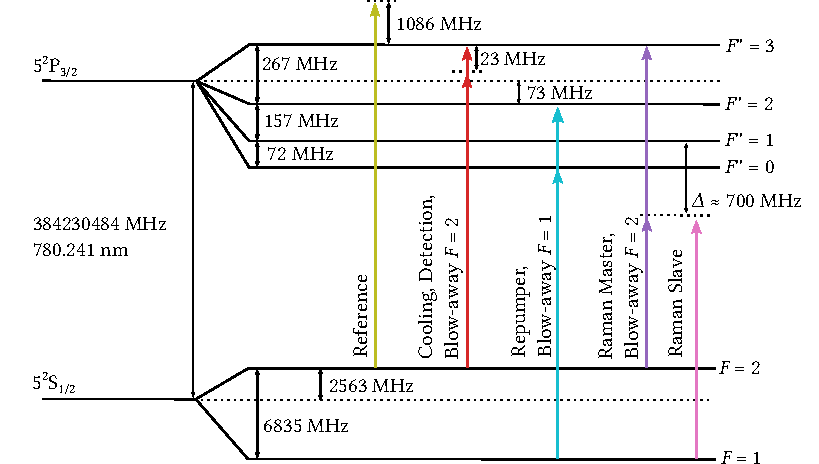
\includegraphics{laser_freqs.pdf}
	\caption{Created with Inkscape}
	\label{fig:laser_freqs}
\end{figure}


This was used to draw fig. \ref{fig:laser_freqs}.




\section{Usage of different mathematics environments}
 {\AmS}-{\LaTeX} is a series of document classes and environments for typesetting mathemtics. The package \code{mathtools} extends this functionality and contains some fixes.

Gl.\,\ref{eq:equation} is a simple equation,
\begin{equation}\label{eq:equation}
	a = b
\end{equation}
Such equations can be split:
\begin{equation}
	\begin{split}
		a& = b+c-d\\
		& \quad + e - f\\
		& = g+h\\
		& = i
	\end{split}
\end{equation}

An expression that spans multiple lines:

\begin{multline}
	a + b + c +d + e + f + a + b + c +d + e + f \\
	+ g + h + i + j + k + l + m + n+ g + h + i + j + k + l + m + n
\end{multline}
And an aligned equation block:
\begin{align}
	a_{11} & = b_{11}          &
	a_{12} & = b_{12}          & \\
	a_{21} & = b_{21}          &
	a_{22} & = b_{22} + c_{22}
\end{align}

\section{More math packages}
Here, we show the usage of some other packages.
\subsection{Differential equations}
With \code{propd} it is possible to typeset differential equations and operators:
\begin{gather}
	\od{y}{x}\\
	\od[2]{u}{x} = -\omega^2 u\\
	\pd{u}{t} = 6u \pd{u}{x} - \pd[3]{u}{x}\\
	\pd{u}{x,x,t}\\
	\pd{}{z}{x+y}\\
	\pd{!}{x}
\end{gather}

\subsection{Chemical formulae}
The package \code{mhchem} is useful to typeset chemical formulae, like \ce{^{235}_{92}U}.

\subsection{Bras and Kets}
For quantum mechanics, use the \code{braket} package:
Quantenmechanik:
\begin{gather}
	\bra{\Phi}\\
	\ket{\Psi}\\
	\braket{\psi|\hat{H}|\phi}
\end{gather}

\subsection{Units}
\code{siunitx} is very useful. It typesets units upright and keeps the appropriate spacing to the value. It is also convenient to specify uncertainties. Here are some examples:

\begin{gather}
	\hbar = \SI[separate-uncertainty=false]{6.62606957(29)e-34}{\joule\second}\\
	g = \SI{9.81(1)}{\meter \per \s^2}\\
	\pi \equiv 3\\
	i \neq \i\\
	e = \SI{1.60217657e-19}{\coulomb}\\
	\e \approx \num{2.71828}\\
\end{gather}

Test of micro symbol: with $\SI{123}{\micro\meter}$ and without \SI{123}{\micro\meter} math environment.
\cleardoublepage
\chapter{Citations, bibliography and tables}\label{ch:conclusion}

\section{Citations and bibliography}
This template uses \code{biblatex}. It allows you to cite titles and authors, i.e. \citetitle{freierMobileQuantumGravity2016} was written by \citeauthor{freierMobileQuantumGravity2016}. Depending on context, either the \code{textcite} command, \textcite{schkolnikEffectWavefrontAberrations2015}, or the \code{parencite} command, \parencite{schkolnikEffectWavefrontAberrations2015}, is used.


\section{Tables}
The two basic rules for nice looking tables are:
\begin{enumerate}
    \item Never use vertical lines.
    \item Never use double lines.
\end{enumerate}
More rules can be find in the \code{booktabs} documentation.


Table \,\ref{tab:tabelle} show the use of \code{threeparttable} which allows to use footnotes inside tables. In addition column style provided by \code{siunitx} is demonstrated.

\begin{table}[htb]
    \centering
    \caption[Usage of \texttt{table}. This shows up in the list of tables]{Note that $E_\text{tot,1}$ and $E_\text{tot,2}$ yield the same result even though they are typeset differently in the source code.}
    \label{tab:tabelle}
    \begin{threeparttable}
        \sisetup{
            table-align-text-post = false
        }
        \begin{tabular}{
                S[table-format = 2.2]
                c
                S[table-format = 2.1(1),separate-uncertainty = true]
                S[table-format = 2.1(1),separate-uncertainty = true]
                S[table-format = 4.2(1),separate-uncertainty = false]
                S[table-format = 3.1,round-mode=places,round-precision=1]
            }
            \toprule
            {$N_{\text{particles,min}}$}                  &
            {This}                                        &
            {$E_\text{tot,1}$ / \si{\giga \electronvolt}} &
            {$E_\text{tot,2}$ / \si{\GeV}}                &
            {$F$ / \si{\newton}}                          &
            {${N'}$}                                                                                             \\
            \midrule
            10.14\tnote{a}                                & is       & 18.3(2) & 18.3+-0.2 & 4018.95(3) & 282.25 \\
            11.54                                         & just     & 18.4(3) & 18.4+-0.3 & 3991.32(4) & 246.45 \\
            12.34                                         & centered & 10.4(2) & 10.4+-0.2 & 3981.19(2) & 230.78 \\
            13.63\tnote{**}                               & text.    & 12.2(6) & 12.2+-0.6 & 3976.35(3) & 221.18 \\
            \bottomrule
        \end{tabular}
        \begin{tablenotes}
            \small{\item[a] This is a footnote}
            \small{\item[**] Little stars also work}
        \end{tablenotes}
    \end{threeparttable}
\end{table}


\pagestyle{plain}
\appendix
\cleardoublepage
\chapter{List of Zernike polynomials}\label{app:zernike}

\begin{center}
\begin{longtable}{cll}
    \caption{Eine mehrseitige Tabelle.}
    \label{tab:zernike}\\
\toprule
{Index $j$} & {Zernike polynomial $Z_j(\theta,\rho)$} & {optical aberration}  \\ 
\midrule
    \endfirsthead
    \caption[]{(continued)}\\
\toprule
{Index $j$} & {Zernike polynomial $Z_j(\theta,\rho)$} & {optical aberration}  \\ 
\midrule
    \endhead
0     &   $ 1 $                                                                     &  piston     \\
1     &   $ \rho \cos \theta $                                                      &  $x$ tilt \\
2     &   $ \rho \sin \theta $                                                      &  $y$ tilt \\
3     &   $ 2\rho^2 - 1 $                                                           &  defocus \\
4     &   $ \rho^2 \cos 2 \theta $                                                  &  astigmatism in \SI{0}{\degree} \\
5     &   $ \rho^2 \sin 2 \theta $                                                  &  astigmatism in \SI{45}{\degree} \\
6     &   $ (3 \rho^3 - 2 \rho) \cos \theta$                                        &  coma in \SI{0}{\degree} \\
7     &   $ (3 \rho^3 - 2 \rho) \sin \theta $                                       &  coma in \SI{90}{\degree} \\
8     &   $ 6 \rho^4 - 6 \rho^2 + 1 $                                               &  spherical aberration \\
9     &   $ \rho^3 \cos 3 \theta $                                                  &  trefoil in \SI{0}{\degree} \\
10    &   $ \rho^3 \sin 3 \theta $                                                  &  trefoil in \SI{30}{\degree} \\
11    &   $ (4\rho^4 - 3 \rho^2)\cos 2 \theta $                                     &  astigmatism (5) in \SI{0}{\degree} \\
12    &   $ (4\rho^4 - 3 \rho^2)\sin 2 \theta $                                     &  astigmatism (5) in \SI{45}{\degree} \\
13    &   $ (10 \rho^5 - 12 \rho^3 + 3 \rho)\cos\theta $                            &  coma (5) in \SI{0}{\degree} \\
14    &   $ (10 \rho^5 - 12 \rho^3 + 3 \rho)\sin\theta $                            &  coma (5) in \SI{45}{\degree} \\
15    &   $ 20 \rho^6 - 30 \rho^4 + 12\rho^2 - 1 $                                  &  spherical aberration (5) \\
16    &   $ \rho^4 \cos 4 \theta $                                                  &  trefoil (7) in \SI{0}{\degree} \\
17    &   $ \rho^4 \sin 4 \theta $                                                  &  trefoil (7) in \SI{22.5}{\degree} \\
18    &   $ (5 \rho^5 - 4 \rho^3)\cos 3 \theta $                                    &  trefoil (7) in \SI{30}{\degree} \\
19    &   $ (5 \rho^5 - 4 \rho^3)\sin 3 \theta $                                    &  trefoil (7) in \SI{52.5}{\degree} \\
20    &   $ (15\rho^6 - 20 \rho^4 + 6 \rho^2)\cos 2 \theta $                        &  astigmatism (7) in \SI{0}{\degree} \\
21    &   $ (15\rho^6 - 20 \rho^4 + 6 \rho^2)\sin 2 \theta $                        &  astigmatism (7) in \SI{45}{\degree} \\
22    &   $ (35 \rho^7 - 60 \rho^5 + 30 \rho^3 - 4 \rho)\cos\theta $                &  coma (7) in \SI{0}{\degree} \\
23    &   $ (35 \rho^7 - 60 \rho^5 + 30 \rho^3 - 4 \rho)\sin\theta $                &  coma (7) in \SI{90}{\degree} \\
24    &   $ 70 \rho^8 - 140 \rho^6 + 90 \rho^4 - 20 \rho^2 + 1 $                    &  spherical aberration (7) \\
25    &   $ \rho^5 \cos 5 \theta $                                                  &  quintuple trefoil (9) in \SI{0}{\degree} \\
26    &   $ \rho^5 \sin 5 \theta $                                                  &  quintuple trefoil (9) in \SI{18}{\degree} \\
27    &   $ (6\rho^6 - 5 \rho^4)\cos 4 \theta $                                     &  quadruple trefoil (9) in \SI{0}{\degree} \\
28    &   $ (6\rho^6 - 5 \rho^4)\sin 4 \theta $                                     &  quadruple trefoil (9) in \SI{22.5}{\degree} \\
29    &   $ (21\rho^7 - 30 \rho^5 + 10\rho^3 )\cos 3\theta $                        &  quadruple trefoil (9) in \SI{0}{\degree} \\
30    &   $ (21\rho^7 - 30 \rho^5 + 10\rho^3 )\sin 3\theta $                        &  quadruple trefoil (9) in \SI{30}{\degree} \\
31    &   $ (56\rho^8 - 105\rho^6 + 60\rho^4 - 10\rho^2 $                           &  astigmatism (9) in \SI{0}{\degree} \\
32    &   $ (56\rho^8 - 105\rho^6 + 60\rho^4 - 10\rho^2 $                           &  astigmatism (9) in \SI{45}{\degree} \\
33    &   $ (126 \rho^9 - 280 \rho^7 + 210 \rho^5 - 60\rho^3 + 5 \rho)\cos\theta $   & coma (9) in \SI{0}{\degree} \\
34    &   $ (126 \rho^9 - 280 \rho^7 + 210 \rho^5 - 60\rho^3 + 5 \rho)\sin\theta $   & coma (9) in \SI{90}{\degree} \\
35    &   $ 252 \rho^{10} - 630 \rho^8 + 560 \rho^6 - 210 \rho^ 4 + 30 \rho^2 - 1 $  & spherical aberration (9) \\
\bottomrule
\end{longtable}
\end{center}

\chapter*{Publications}\label{app:publications}

\begin{refsection}
	
	\section*{Print}
	\begin{itemize}
		\AtNextCitekey{\defcounter{maxnames}{99}}
		\item \fullcite{schkolnik_effect_2015}
		\AtNextCitekey{\defcounter{maxnames}{99}}
		\item \fullcite{freier_mobile_2016}
		\AtNextCitekey{\defcounter{maxnames}{99}}
		\item \fullcite{hu_mapping_2017} 
		\AtNextCitekey{\defcounter{maxnames}{99}}
		\item \fullcite{hu_observation_2018}
		\AtNextCitekey{\defcounter{maxnames}{99}}
		\item \fullcite{wiegand_single-laser_2019}
		\AtNextCitekey{\defcounter{maxnames}{99}}
		\item \fullcite{canuel_elgar_2019} 
	\end{itemize}
	
	\section*{Oral and Poster Presentations}
	Only those presentations are listed where the thesis author is first  author and presenter.
	\subsection*{Oral}
	\begin{itemize}
		\item Deutsche Physikalische Gesellschaft (DPG) Frühjahrstagung, Heidelberg, Germany (2015)
		\item European Geosciences Union (EGU) General Assembly, Vienna, Austria (2017)
	\end{itemize}
	\subsection*{Poster}
	\begin{itemize}
		\item Frontiers of Matter Wave Optics (FOMO), Chania, Greece (2014)
		\item Deutsche Physikalische Gesellschaft (DPG) Frühjahrstagung, Hannover, Germany (2016)
		\item Frontiers of Matter Wave Optics (FOMO), Arcachon, France (2016), awarded with prize for \emph{Best Poster Presentation} 
	\end{itemize}
	
\end{refsection}
\printbibliography
   \label{app:bibliography} 

\cleardoublepage
\begin{german}
\chapter*{Danksagung}
   An dieser Stelle möchte ich meiner Mutti danken.
\end{german}
\begin{german}
\chapter*{Selbstständigkeitserklärung}
\thispagestyle{empty}
   Hiermit erkläre ich, dass ich die vorliegende Arbeit selbstständig und nur unter Zuhilfenahme der angegebenen Quellen und Hilfsmittel verfasst habe.
\bigskip
 
\noindent\textit{\mylocation, \mytime}

\smallskip

\begin{flushright}
    \begin{tabular}{m{5cm}}
        \\ \hline
        \centering\myname \\
    \end{tabular}
\end{flushright}
\end{german}
\end{document}